\subsection{Probability Based Tiling}
\subsubsection{Motivation}
As discussed in section \ref{sec:UnifTiling}, uniform tiling optimizes tree walks assuming that all paths in the tree from root to leaf are equally likely. 
However, we find that this is not always the case. We performed inference on the complete training set of each of our benchmarks and measured how many
times each leaf was reached. While for some benchmarks all leaves are roughly equally likely, for others, a small number of leaves are extremely likely 
while the rest aren't reached often. We call trees with a small number of extremely likely leaves \textbf{\emph{skewed}}.
\begin{figure}
    \centering
    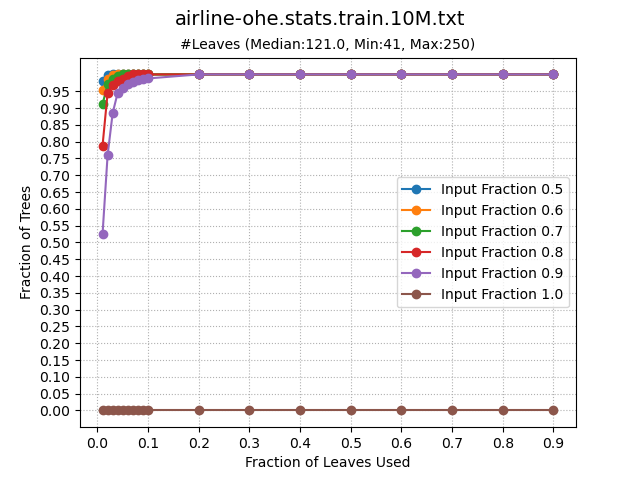
\includegraphics[width=\linewidth]{figures/airline-ohe.stats.train.txt.png}
    \caption{Statistical profile for airline-ohe}
    \label{Fig:AirlineOHEStats}
\end{figure}
\begin{figure}
    \centering
    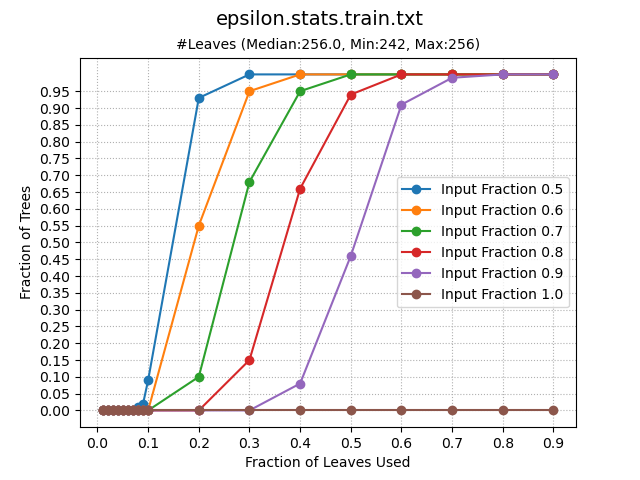
\includegraphics[width=\linewidth]{figures/epsilon.stats.train.txt.png}
    \caption{Statistical profile for epsilon}
    \label{Fig:EpsilonStats}
\end{figure}
Figures \ref{Fig:AirlineOHEStats} and \ref{Fig:EpsilonStats} show this. Each line in these graphs corresponds to a fixed fraction of the input (say $f$). 
A point on a line at coordinate $(x, y)$ means that $y$ percent of trees in the model could handle a fraction $f$ of all training inputs with $x$ percent of 
leaves. \TODO{Explain with a specific point in one of the graphs}
Figure \ref{Fig:AirlineOHEStats} shows that very few leaves are reached for a very large fraction of inputs for the benchmark airline-ohe. 
This means that a small fraction of leaves are very likely. On the other hand,
figure \ref{Fig:EpsilonStats} shows that a large fraction of trees need a large fraction of their leaves to handle any fraction of the test input 
for the benchmark epsilon. One other observation we made is that most models have some skewed trees while the rest of the trees have equally likely leaves.
\TODO{AP Define a term for trees with roughly equally likely leaves.} We design the probability based tiling algorithm to take advantage of this property 
of decision tree ensembles. 
\TODO{This section needs to be rewritten. Define ``leaves covering inputs'' to clarify the presentation.}

\subsubsection{Notation}
In order to formulate the probability based tiling algorithm as an optimization problem, we define the following.
\begin{enumerate}
    \item For every leaf $l \in L$, we define $p_l$ as the probability that the leaf $l$ is reached.
    \item For each node $n \in V$, we define the absolute probability $p_v$ as
    \begin{equation}
        p_v = \begin{cases}
        p_l &\text{if $l \in L$}\\
        p_{left(v)} + p_{right(v)} &\text{otherwise}
        \end{cases}
    \end{equation}
    \item For any tree $T$, $\mathcal{C}(T)$ represents the set of all valid tilings of $T$.
    \item For every $v \in V$, we define $S_v$ as the subtree rooted at $v$.
    \item For every $v \in V$, we define $L_v$ as the set of leaves of $S_v$.
    \item For a every tile $T_i$, we define $root(T_i)$ as the node $v \in T_i$ such that $v$ has no incoming edges from any other node $u \in T_i$.
    \item For a tile $T_i$, $out(T_i) \subseteq E$ is the set of edges $(u, v)$ such that $u \in T_i$ and $v \notin T_i$.
\end{enumerate}

\subsubsection{The Optimization Problem}

%We assume that we are given the probabilities of each leaf node of the decision tree (these can easily be computed using the training data). For every leaf $l \in L$, we %are given the probability $p_l$ that the leaf $l$ is reached. 

We observe that the latency of one tree walk is proportional to the number of tiles that need to be evaluated to reach the leaf.
Therefore, the average inference latency can be modelled as the expected number of tiles that are evaluated to compute one tree prediction. More formally, the problem is to find a tiling $\mathcal{T}$ such that the following objective is minimized.
\[
    \min_{\mathcal{T} \in \mathcal{C}(T)}{\sum_{l \in L} p_l.depth_{\mathcal{T}}(l)}
\]
where the minimization is over all valid tilings $\mathcal{T}$ of the tree $T$, $depth_{\mathcal{T}}(l)$ is the depth of the leaf $l$ given tiling ${\mathcal{T}}$.

The constraints on the optimization are the constraints listed in Section \ref{sec:ValidTiling}. 
The above optimization problem can be solved optimally using dynamic programming. We leave this out in the interest of space. 
Instead, we use the simple greedy algorithm listed in algorithm \ref{Alg:GreedyTilingAlgo} to construct a valid tiling given the node probabilities.
The algorithm starts at the root and greedily keeps adding the most probable legal node to the current tile until the maximum tile size is reached.
Subsequently, the tiling procedure is recursively performed on all nodes that are destinations for edges going out of the constructed tile.

% \subsubsection{Dynamic Programming Formulation}


% For any node $v \in V$, we define
% \[
%     cost(v, \mathcal{T}) = \sum_{l \in L_v} p(l | v).depth_{\mathcal{T}}(l)
% \]
% where $\mathcal{T} \in \mathcal{C}(T_v)$.

% Then, the objective function, for the tree $T_v$, can be rewritten as 
% \[
%     opt\_cost(v) = \min_{\mathcal{T} \in \mathcal{C}(T_v)}{cost(v, \mathcal{T})}
% \]

% The objective function can then be rewritten in the following recursive form.
% \[
%     opt\_cost(v) = \min_{T_0 \in TileShapes(n_t, v)}{1 + \sum_{(n_1, n_2) \in out(T_0)} p(n_1 | v)p(n_2 | n1)opt\_cost(n_2)}
% \]
% where $TileShapes(n_t, v)$ is the set of all tile shapes of size $n_t$ with root $v$. A straight forward substitution argument shows why the solution to the subproblems (tiling all sub-trees) needs to to be optimal. The objective is now in a form that can solved using
% dynamic programming. 

% \subsubsection{Greedy Algorithm}

% Intuitively, it seems like the following greedy algorithm also gives the optimal tiling. The algorithm starts at the root and greedily keeps adding the most probable node to the current tile until the maximum tile size is reached.
\begin{algorithm}
    \caption{Greedy Probability Based Tree Tiling}
    \label{Alg:GreedyTilingAlgo}
    \begin{algorithmic}
        \Procedure{TileTree}{$T = (V, E, r)$, $n_t$} 
            \If {$r \in L$}
                \State \textbf{return} $\{ r \}$
            \EndIf
            \State $Tile \leftarrow \{ r \}$
            \While{$|Tile| < n_t$}
                \State $e = (u,v) \in Out(Tile)$ st $p(v)$ is max and $v \notin L$
                \If{$e = \emptyset$}
                    \State \textbf{break}
                \EndIf
                \State $Tile = Tile \cup \{ v \}$
            \EndWhile
            \State $Tiles =  \{ Tile \}$
            \For{$(u,v) \in Out(Tile)$}
                \State $Tiles \leftarrow Tiles \cup TileTree(S_v, n_t)$
            \EndFor
            \State \textbf{return} $Tiles$
        \EndProcedure
    \end{algorithmic}
\end{algorithm}

% Talk about problems with increasing number of tile shapes and only performing such tiling on skewed trees
When we tried to apply algorithm \ref{Alg:GreedyTilingAlgo} on all trees in our benchmarks, we found
that even minor variations in probability caused the tiling algorithm to generate a large 
number of tile shapes. This in turn caused a loss in performance because the large size of the 
lookup table needed (section \ref{sec:LookupTable}) caused increased L1 cache misses. In order to 
alleviate this, we only perform probability based tiling on trees that are skewed. We say a tree is
skewed if a small fraction of leaves, say $\alpha$, cover a large fraction of training inputs, say $\beta$.
We only perform probability based tiling on skewed trees and fall back to uniform tiling otherwise. 
In our experiments we use $\alpha=0.05$ and $\beta=0.9$. 

\subsubsection{Code Generation}
As probability based tiling pulls the most probable leaves of a decision tree nearest the root, it poses 
some implementation challenges. By design, the tiling process makes the tree of tiles 
imbalanced. Therefore, the simple array based representation described in section \ref{sec:ArrayBased}
cannot be used because of the memory footprint blow up (a large part of the tree is empty, but would 
need to be allocated). On the other hand, the sparse representation in section \ref{sec:SparseRep} adds 
an extra hop for leaves that have non-leaf siblings. But this would mean that we add extra hops for 
the most probable leaves after probability based tiling. To address these problems, Treebeard peels 
the tree walk and specializes the leaf checks at higher levels to avoid the extra hop. Currently, 
we determine the maximum depth of leaves needed to cover 90 percent of the inputs and peel the tree 
walk by as many iterations. For example, consider the case where leaves until depth 2 are needed to 
cover 90 percent of the training input. Then, Treebeard generates the following IR. 

\begin{lstlisting}{style=c++}
    // ...
    tree = getTree(forest, t)
    node = getRoot(tree)
    node = traverseTreeTile(tree, node, rows[i])
    if (isLeafTile(node)) {
        treePrediction = getLeafValue(tree, node)
    } else {    
        node = traverseTreeTile(tree, node, rows[i])
        if (isLeafTile(node)) {
            treePrediction = getLeafValue(tree, node)
        } else {    
            // Loop based traversal 
        }
    }
    treePrediction = getLeafValue(tree, node)
    // ...
\end{lstlisting}

The if statements check whether a node is a leaf tile and hence avoid the extra hop. The memory 
requirement is also not increased because only a small fraction of leaves are represented as full tiles.
While walk peeling is used to improve the performance of probability based tiling by specializing leaf tests,
the transformation is by itself general and can be used in different contexts. For example, it could be used 
to elide leaf checks until a depth $d$ is reached if we know all leaves are at a depth greater than $d$. 

One other issue that the code generator needs to handle is that walks of different trees in the same ensemble may 
need to be peeled to different depths. In order to handle this, trees are reordered so that all trees 
with equal peeling depth are grouped together and the loops in the IR are fissed so that tree walks 
for these groups of trees can be specialized differently. This is very similar to the code generation strategy
used for uniform tiling.

